\documentclass[11pt]{article}
\usepackage[margin=1in]{geometry}
\usepackage{amsmath,amssymb,amsthm,mathtools}
\usepackage{booktabs,tabularx}
\usepackage{graphicx}
\usepackage[hidelinks]{hyperref}
\usepackage{xcolor}
\usepackage{enumitem}
\setlist{nosep,leftmargin=*}

\newtheorem{theorem}{Theorem}
\newtheorem{proposition}[theorem]{Proposition}
\newtheorem{lemma}[theorem]{Lemma}
\theoremstyle{definition}
\newtheorem{prediction}{Prediction}
\theoremstyle{remark}
\newtheorem{remark}[theorem]{Remark}

\newcommand{\E}{\mathbb{E}}
\newcommand{\Var}{\mathrm{Var}}
\newcommand{\Cov}{\mathrm{Cov}}
\newcommand{\I}{\mathcal{I}}
\newcommand{\src}[1]{\textsf{[#1]}}
\newcommand{\answer}[1]{\par\smallskip\noindent\fbox{\parbox{\dimexpr\linewidth-2\fboxsep-2\fboxrule}{\textbf{Answer.} #1}}\par\smallskip}

\title{When Can a Bandit Trust Correlation?\\[2pt]
\large Certified Pooling and Persistent Dynamics for Correlated Arms on the Web}
\author{Working long version, 9 October 2026 (revision 2)\\
\small Compiled from the \texttt{dependent\_mab} repository, to be condensed into a WWW 2027 submission}
\date{}

\begin{document}
\maketitle

\begin{abstract}
A short-video platform filling a daily trending slot faces arms that are correlated in two ways: videos watched by the same people tend to be liked by the same people, and a video's engagement today predicts its engagement for days. Platforms hold many graphs that seem to encode such structure, from co-engagement logs to social networks to hyperlinks, and graph bandits invite the learner to pool information along them. We ask when that trust is warranted.

We model every reward as $f_{i,t}=\mu_i+z_{i,t}$, with a \emph{mean channel} (long-run appeal $\mu$, restricted by a graph certificate) and a \emph{fluctuation channel} (persistent deviations $z$ with graph-correlated shocks), and organize theory and evidence around four questions. \textbf{Which correlation is real?} On KuaiRec, collaborative graphs carry personal taste while social, profile and location graphs carry almost none; for fluctuations, hyperlinks carry shock correlation five times that of random pairs, but only when the arms span communities with different rhythms. \textbf{How can a learner pool safely?} Certified pooling gains exactly where its theory says it should: the median regret ratio to UCB1 falls from 0.84 to 0.40 as the share of rejectable components rises. Uncertified pooling fails precisely when a best item sits in a weaker community, which happens on informative graphs and never on random ones. \textbf{What breaks when rewards persist?} We prove that certified pooling stays valid under persistent, correlated, restless sampling when its confidence sets come from an exact innovation regression, give tight scalar certificates for independent and correlated shocks, and show that iid certificates fail under bursty exposure; the predicted variance inflation (3.5--4.4$\times$) matches observed violation rates of 85--93\%, while innovation certificates are never violated. \textbf{How should a learner act on persistent fluctuations?} Modelling dynamics cuts regret by 24--43\% against iid Thompson sampling on both platforms; heavy exploration of persistent uncertainty pays only when arms receive many observations and the top is well separated, while mild optimism helps where priors are weak or rankings turn over; and a graph improves the fluctuation model only when shocks are community-specific, changing decisions by at most 3\% even then, because long-run levels rather than shocks decide which items lead.
\end{abstract}

\tableofcontents
\newpage

%=====================================================================
\section{Introduction}
%=====================================================================

\paragraph{A running example.} Every day a short-video platform shows ten videos in a trending slot. Two facts shape the decision. First, videos are related: those watched by the same audience tend to be enjoyed by the same audience, so evidence about one video is evidence about its neighbours. Second, engagement persists: a video's completion rate today predicts tomorrow's, and shocks such as a holiday or an outage hit many videos at once. The platform also holds many graphs that might encode the first fact (co-engagement, matrix-factorization neighbours, creator links, tags, a social network) and must decide which to use, if any.

\paragraph{Two ways to get it wrong.} A learner can \emph{trust correlation that is not there}: pooling along a graph whose neighbourhoods do not share appeal biases estimates, and in the worst case leads to linear regret. Or it can \emph{ignore that rewards persist}: confidence statements built for independent rewards are too narrow when consecutive observations of an item move together, so decisions that rely on them, such as dropping an item for good, go wrong. Both mistakes are easy to make on the web, where graphs are by-products rather than designed priors and where exposure is bursty: the same items fill a slate day after day.

\paragraph{Model.} We write every reward as $f_{i,t}=\mu_i+z_{i,t}$. The \emph{mean channel} restricts long-run appeal $\mu$ with a graph certificate; the \emph{fluctuation channel} lets deviations $z$ follow an autoregression with graph-correlated shocks. Graphs are a tool for encoding correlation in either channel, not the object of study.

\paragraph{Four questions.} Table~\ref{tab:roadmap} lists the questions, the theory that makes each testable, and the answer the evidence gives. Each of Sections~\ref{sec:q1}--\ref{sec:q4} follows the same pattern: what theory says, what it predicts, what we find, and what it means.

\begin{table}[t]\centering\small
\begin{tabularx}{\linewidth}{p{2.7cm}p{4.2cm}X}
\toprule
Question & Theory that makes it testable & Answer from the evidence \\
\midrule
Q1. Which correlation is real? (\S\ref{sec:q1}) & Graph energy relative to gaps; smoothing changes the argmax; random graphs act as uniform shrinkage & Collaborative graphs carry taste; social, profile, location graphs barely do. Fluctuations: links carry shocks only across communities with different rhythms. \\
Q2. How can a learner pool safely? (\S\ref{sec:q2}) & Certified pooling regret; gains only from components with width below gap & Gains track the rejectable share (0.84 $\to$ 0.40 of UCB1). Uncertified pooling fails when a best item sits in a weaker community. Practical certificates remain the bottleneck. \\
Q3. What breaks when rewards persist? (\S\ref{sec:q3}) & Innovation regression; certificates B1, B1$'$, B1$''$; failure result B2 & iid certificates fail under bursty exposure as B2 predicts (85--93\% of runs); innovation certificates are never violated, at comparable regret. \\
Q4. How should a learner act on persistent fluctuations? (\S\ref{sec:q4}) & Innovation lower bound; exploration should target uncertainty that persists & Modelling dynamics: $-24$ to $-43\%$ regret. Heavy exploration needs many observations per arm and clear gaps; mild optimism helps when rankings move. Graph-shrunk shocks matter only when fluctuations decide the ranking. \\
\bottomrule
\end{tabularx}
\caption{Roadmap: four questions, the theory behind each, and the answers.}\label{tab:roadmap}
\end{table}

\paragraph{Contributions.}
\begin{enumerate}
\item A two-channel model of correlated arms that contains iid bandits, static graph bandits and restless autoregressive bandits as special cases, and separates what a graph can encode (\S\ref{sec:model}).
\item \textbf{Theory bridging the channels} (\S\ref{sec:q3}, proofs in Appendix~\ref{app:proofs}): certified pooling is valid under persistent, correlated, restless sampling when built on an exact innovation regression (B1); tight scalar certificates for independent shocks (B1$'$) and, by iterated nuisance plug-in, for correlated shocks (B1$''$); a quantitative failure result for iid certificates (B2); and long-run substitution of the mean-channel constants (B3).
\item \textbf{Predictions tested against data.} Each theoretical statement yields a prediction that we test: certified gains track rejectable components (\S\ref{sec:q2}); uncertified pooling fails through dilution (\S\ref{sec:q2}); B2's variance inflation matches observed violation rates (\S\ref{sec:q3}); exploration pays with enough future observations per arm (\S\ref{sec:q4}).
\item \textbf{Measurements on two web platforms} (KuaiRec short video; Wikipedia attention in one and in six communities) and a controlled 100-arm spatiotemporal benchmark, including a hypothesis-driven experiment showing when hyperlinks carry correlated shocks (\S\ref{sec:q1}, \S\ref{sec:q4}).
\end{enumerate}

\paragraph{Provenance.} Results proved in companion manuscripts in the repository are labelled \src{A} (graph alignment and certified pooling), \src{S} (spatiotemporal filtering and confidence), \src{P} (predictive and AR bandits) and \src{N} (a repository note on the selection index). Results first stated here are labelled \src{New}.

%=====================================================================
\section{Setting: two channels of correlation}\label{sec:model}
%=====================================================================

There are $N$ arms. In round $t$ the learner pulls one arm, or a slate $S_t$ of $k$ arms, and observes
\begin{equation}\label{eq:model}
Y_t=\mu_{a_t}+z_{a_t,t}+\xi_t,\qquad z_t=\sum_{r=1}^{p}A_r z_{t-r}+\eta_t,\qquad \eta_t\sim N(0,Q_G),\qquad \xi_t\sim N(0,r).
\end{equation}
Every arm evolves every round (restless); only pulled arms are observed.

\paragraph{Mean channel.} Long-run means $\mu\in[0,1]^N$ are unknown. A graph supplies either a partition $\{C_c\}$ with certified diameters $\varepsilon_c\ge\max_{i\in C_c}\mu_i-\min_{i\in C_c}\mu_i$, or an energy certificate $\mu_c^\top L_c\mu_c\le S_c^2$, which implies diameters through effective resistance \src{A}.

\paragraph{Fluctuation channel.} Deviations persist through $A_r$ and are correlated across arms through $Q_G$, which can be shrunk toward a graph kernel. A shock common to all arms (a holiday) and a shock common to a community (a league's game day) are both correlation; only the second is something a graph can tell apart from a common factor.

\paragraph{Regret.} \emph{Mean regret} $\sum_t(\mu^\star-\mu_{a_t})$ measures learning of persistent appeal. \emph{Dynamic regret} $\sum_t(\max_i f_{i,t}-f_{a_t,t})$ measures tracking of current rewards against an oracle that sees every arm's current value. With slates, both are summed over the slate against the oracle's top $k$.

\paragraph{Special cases.} iid bandits: $A_r=0$, $Q_G$ diagonal, no certificate. Static graph bandits: $A_r=0$ with a mean certificate. Restless AR bandits: no mean certificate. Spectral bandits regularize the mean channel without certifying it.

%=====================================================================
\section{Q1. Which correlation is real?}\label{sec:q1}
%=====================================================================

\subsection{What theory says}

For the mean channel, a graph helps only if long-run appeal is smooth on it relative to the gaps that matter. Two facts sharpen this \src{A,N}. Smoothing on a complete graph shrinks all arms toward a common value and preserves every ranking; smoothing on an informative graph pulls an arm toward its neighbourhood's level, which can change the best arm (the misalignment example: $\mu=(1,0.9,0)$ with arms 1 and 3 linked makes arm 2 best after smoothing). So a graph can be \emph{smoother than chance} and still \emph{unsafe to smooth}. For the fluctuation channel, a graph helps only if shocks are correlated along its edges beyond what a single common factor explains.

\begin{prediction}\label{pred:q1}
(a) Graphs built from collaborative signals align with personal taste more than graphs built from profiles or content. (b) Fixed smoothing on informative graphs changes users' best items more than smoothing on rewired graphs. (c) A graph improves the shock model only if shocks are community-specific.
\end{prediction}

\subsection{Evidence: the mean channel on KuaiRec}

KuaiRec contains a 1,411 user $\times$ 3,327 video matrix that is 99.6\% observed. A larger sparse matrix (7,176 $\times$ 10,728) shares no (user, video) pair with it, so every graph is built leakage-free: user-side signals use only non-evaluation videos and video-side signals only non-evaluation users. We build sixteen graphs (Appendix~\ref{app:data}) and compare each with a degree-preserving rewiring. Table~\ref{tab:align} and Figure~\ref{fig:align} report three measures: a smoothness quotient (Laplacians scaled so a random graph scores about 1), the correlation of neighbours' personal taste after removing each user's activity and each video's popularity, and the cost to each user's best choice of smoothing true means with $(I+10L)^{-1}$.

\begin{table}[t]\centering\small
\resizebox{\linewidth}{!}{%
\begin{tabular}{lcccc}
\toprule
Graph & Side & Quotient (real / rewired) & Personal-taste corr. (real / random) & Choice cost, $\lambda{=}10$ (real / rewired) \\
\midrule
I-mf (factorization) & item & 0.756 / 0.961 & \textbf{0.046} / 0.002 & 0.117 / 0.019 \\
I-coeng (co-engagement) & item & 1.098 / 1.302 & \textbf{0.034} / 0.002 & 0.131 / 0.037 \\
I-cat / I-tag (content) & item & 0.908 / 0.985, 0.943 / 1.010 & 0.010 / 0.002 & 0.099 / 0.079, 0.100 / 0.054 \\
I-coauthor (same creator) & item & 0.805 / 1.006 & 0.004 / 0.002 & 0.040 / 0.184 \\
U-coeng (co-engagement) & user & \textbf{0.649} / 0.791 & \textbf{0.020} / 0.000 & 0.284 / 0.291 \\
U-coauthor, U-coeng-idf & user & 0.761 / 0.871, 0.748 / 0.860 & 0.018 / 0.000 & 0.296 / 0.294 \\
U-mf (factorization) & user & 0.850 / 0.907 & 0.016 / 0.001 & 0.300 / 0.298 \\
U-cotag, U-cotime & user & 0.842 / 0.884, 0.931 / 0.947 & 0.004, 0.003 & 0.299 / 0.297, 0.315 / 0.304 \\
U-geo, U-feat, U-demo & user & 0.946, 0.972, 0.988 & 0.007, 0.006, 0.002 & 0.350, 0.305, 0.328 \\
U-soc (social; 47 edges) & user & not comparable & 0.035 per edge & -- \\
\bottomrule
\end{tabular}}
\caption{KuaiRec: which graphs encode correlated appeal (reward = capped watch ratio, $k=10$).}\label{tab:align}
\end{table}

\begin{figure}[t]\centering
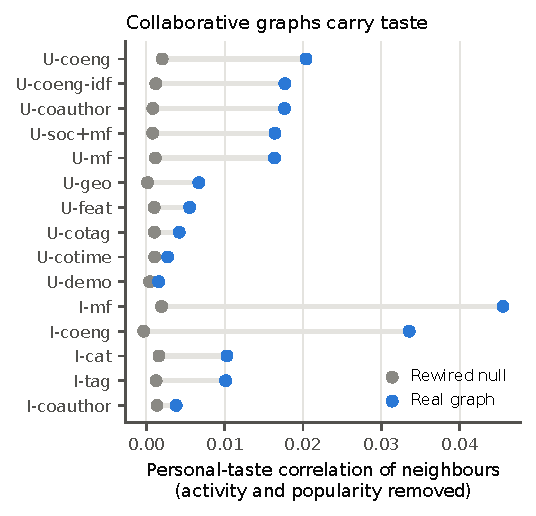
\includegraphics[width=0.5\linewidth]{../figures/f1_alignment.pdf}
\caption{Personal-taste correlation of graph neighbours, real graph against its rewiring.}\label{fig:align}
\end{figure}

\paragraph{Findings.}
\begin{itemize}
\item \emph{Collaborative graphs carry taste} (Prediction~\ref{pred:q1}a). Factorization and co-engagement neighbours agree on personal taste at 17--23 times the random-pair level; tag, category and creator graphs mostly group videos of similar popularity, and their advantage over the rewiring disappears once popularity is removed. Among user graphs, co-engagement is best; profile, location and demographic graphs are close to random. The social graph covers only 80 of 1,411 users. Rankings are stable across $k\in\{5,10,20\}$ and under a binary like-based reward (rank correlation 0.80).
\item \emph{Smoother than chance is not safe to smooth} (Prediction~\ref{pred:q1}b). On item graphs, fixed smoothing costs more of a user's best-choice value on the real graph than on its rewiring (I-mf at $\lambda=10$: 0.117 against 0.019). The rewiring smooths each video toward a random sample of others, which acts like uniform shrinkage; the real graph pulls videos toward their community, which reorders the top. The exception (I-coauthor) makes small cliques of near-identical videos.
\item User graphs are dominated by a shared popularity component: users' rows correlate at 0.38 even for random pairs.
\end{itemize}

\subsection{Evidence: the fluctuation channel on three panels}

Table~\ref{tab:shocks} compares shock correlation along graph edges, along rewired edges and across all pairs, and the held-out likelihood of the innovation covariance under each graph target, on three daily panels: KuaiRec (253 videos, 63 days), Wikipedia programming-language articles (150 articles, 2022--2025) and Wikipedia articles from six communities (NFL, NBA, MLB, Premier League, countries, programming languages; 25 each). The six-community panel was designed after the first two returned a null, to test Prediction~\ref{pred:q1}c directly.

\begin{table}[t]\centering\small
\resizebox{\linewidth}{!}{%
\begin{tabular}{lcccccc}
\toprule
Panel & Graph & Shock corr.: edges / rewired / all & Within / across communities & Held-out log-lik per day: graph / rewired / common factor \\
\midrule
KuaiRec daily & co-engagement & 0.071 / 0.068 / 0.042 & -- & $-323.0$ / $-323.3$ / $\mathbf{-305.7}$ \\
Wikipedia, one domain & hyperlinks & 0.256 / 0.250 / 0.218 & -- & 52.88 / 52.85 / \textbf{53.76} \\
Wikipedia, six domains & hyperlinks & \textbf{0.273} / 0.051 / 0.051 & 0.320 / 0.000 & \textbf{22.16} / 21.67 / 21.92 \\
\bottomrule
\end{tabular}}
\caption{Do graphs carry correlated shocks? Held-out log-likelihood scores AR residuals of a 120-day (Wikipedia) or remaining-days (KuaiRec) window under each innovation-covariance target fitted on the preceding window, averaged over three origins. Domain blocks score 22.13 on the six-domain panel.}\label{tab:shocks}
\end{table}

\paragraph{Findings.}
\begin{itemize}
\item On KuaiRec and on single-domain Wikipedia, shocks are correlated, but through a platform- or domain-wide factor: graph edges are no more correlated than rewired edges, and a common-factor covariance fits held-out shocks best.
\item With six communities, the picture reverses (Prediction~\ref{pred:q1}c). Shocks correlate at 0.32 within a community and 0.00 across; 84\% of hyperlinks stay within a community, so hyperlinked pairs correlate at 0.273 against 0.051 for rewired pairs. Hyperlinks give the best held-out fit at all three origins, matching an oracle community-block graph (22.13).
\end{itemize}

\answer{For long-run appeal, trust collaborative graphs (factorization, co-engagement) and treat profile, location, social and content graphs as popularity signals. Even a good graph is not safe to smooth with a fixed strength. For fluctuations, a graph adds information only when the arms span communities with different rhythms; within one community, a common factor captures the shared shocks.}

%=====================================================================
\section{Q2. How can a learner pool safely?}\label{sec:q2}
%=====================================================================

\subsection{What theory says}

\paragraph{Certified pooling \src{A}.} SP-UCB keeps an arm upper bound $u_i=\bar Y_i+b(n_i)$, $b(n)=\sigma\sqrt{2\ell/n}$, and a pooled component bound, selects the component maximizing $U_c=\min\{\max_{i\in C_c}u_i,\ \hat p_c+b(N_c)+\varepsilon_c\}$ and pulls its best arm.

\begin{theorem}[Alignment-sensitive regret \src{A}]\label{thm:spucb}
With valid certificates, with probability at least $1-\delta$,
$\mathcal R_T\le\sum_{c\in\mathcal O}A_c+\sum_{c\notin\mathcal O}\min\{A_c,H_c\}$, where $A_c=\sum_{i\in C_c:\Delta_i>0}(\Delta_i+8\sigma^2\ell/\Delta_i)$ is the cost of exploring the component arm by arm and $H_c=(\Gamma_c+\varepsilon_c)(1+8\sigma^2\ell/(\Gamma_c-\varepsilon_c)^2)$ is the cost of rejecting it as a whole, finite only when its width $\varepsilon_c$ is below its gap $\Gamma_c$.
\end{theorem}

Graph geometry, not diameter, sets the value of a certificate: a path and a clique with identical diameters and energy budgets differ in information cost by a factor growing with the component size, and the cost of loosening a certificate grows with the resistance radius \src{A}. A certified Laplacian comparison $(1-\eta)L\preceq\hat L\preceq(1+\eta)L$ allows estimated graphs by inflating the energy radius to $\sqrt{1+\eta}\,S$ \src{A}.

\begin{prediction}\label{pred:q2}
(a) Certified pooling gains only through components whose width is below their gap: gains should rise with the share of such \emph{rejectable} components. (b) Pooling with zero width (no certificate) fails when the optimal arm's component has a lower average than another component, since the pooled bound then rejects the optimal component; larger optimal components dilute more. (c) Average gains come mostly from shrinkage, so rewired graphs should do about as well on average.
\end{prediction}

\subsection{Evidence}

\paragraph{Design (Setting A).} For each of 60 test users, 300 videos are sampled and each item graph is rebuilt on them; SP-UCB uses a 20-component spectral partition; rewards are Bernoulli with the user's true means; $T=20{,}000$; common random numbers across policies. Setting A v2 repeats this with KL-based bounds (30 users $\times$ 2 subsets) and adds practical certificates.

\begin{table}[t]\centering\small
\resizebox{\linewidth}{!}{%
\begin{tabular}{lccc}
\toprule
Share of suboptimal components rejectable (oracle certificate) & Instances & Median SP-UCB / UCB1 & Interquartile range \\
\midrule
$\le$ 40\% & 54 & 0.84 & 0.78--0.91 \\
40--60\% & 67 & 0.73 & 0.63--0.79 \\
60--80\% & 119 & 0.52 & 0.41--0.61 \\
$>$ 80\% & 120 & 0.40 & 0.30--0.83 \\
\midrule
\multicolumn{4}{l}{Spearman correlation of the rejectable share with the log ratio: $-0.48$ ($p\approx10^{-22}$)} \\
\bottomrule
\end{tabular}}
\caption{Certified gains track the theorem's rejectability condition (Prediction~\ref{pred:q2}a).}\label{tab:rejectable}
\end{table}

\begin{figure}[t]\centering
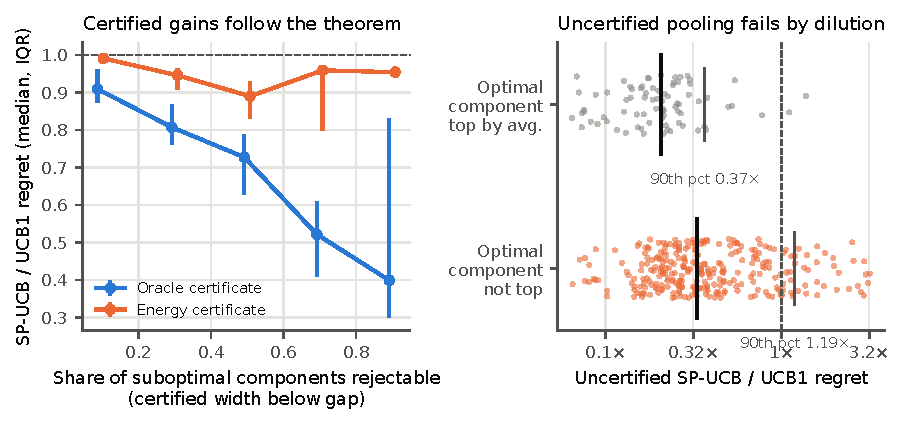
\includegraphics[width=\linewidth]{../figures/f2_pooling_bridge.pdf}
\caption{Left: certified gain against the share of rejectable components (median and interquartile range). Right: uncertified pooling, split by whether the optimal arm's component is the top component by average; failures (ratio above 1) occur almost only when it is not.}\label{fig:pooling}
\end{figure}

\paragraph{Findings.}
\begin{itemize}
\item \emph{Gains follow the theorem} (Prediction~\ref{pred:q2}a; Table~\ref{tab:rejectable}, Figure~\ref{fig:pooling}). The median regret ratio of oracle-certified SP-UCB to UCB1 falls from 0.84 when at most 40\% of suboptimal components are rejectable to 0.40 when more than 80\% are. Energy certificates are wider (energy-to-gap ratio about 5 on every graph) and rarely make components rejectable: in 268 of 360 instances fewer than 40\% are, and their median gain is only 2--11\% in every bin. The widest bin for oracle certificates ($>80\%$) has a long upper tail (75th percentile 0.83), driven by graphs with many tiny components.
\item \emph{Uncertified pooling fails by dilution} (Prediction~\ref{pred:q2}b). When the optimal arm's component is the top component by average, zero-width pooling is safe (median 0.21$\times$ UCB1, 90th percentile 0.37$\times$). When it is not, the 90th percentile rises to 1.19$\times$; the size of the optimal component is the strongest predictor (Spearman 0.56). Failures concentrate on graphs that make communities differ: 38\% of users fare worse than UCB1 on the creator graph, 15\% on categories, 2\% on factorization, and none on the rewired graph. Informative graphs are exactly the ones that make uncertified pooling dangerous, because they make component averages differ.
\item \emph{Average gains are shrinkage} (Prediction~\ref{pred:q2}c). SpectralUCB at $\lambda=10$ regrets $0.697\times$ UCB1 on I-mf and $0.695\times$ on its rewiring; spectral Thompson sampling $0.611\times$ against $0.610\times$. Uncertified pooling with KL bounds is best on average ($0.67\times$ KL-UCB) and does as well on the rewired graph. In Setting B (users arrive at random, 300 users $\times$ 100 videos), shrinking toward the population mean cuts regret 27\% and no user graph beats it; user pooling without a certificate is 39\% worse than none, with an oracle certificate 6\% better.
\end{itemize}

\begin{table}[t]\centering\small
\resizebox{\linewidth}{!}{%
\begin{tabular}{lcccc}
\toprule
SP-KLUCB certificate (I-mf) & Regret / KL-UCB (mean / 90th pct.) & Components valid & Mean width \\
\midrule
Oracle (true within-component range) & 0.78 / 1.05 & 100\% & 0.36 \\
Per-user calibrated, 75th percentile & 0.88 / 1.05 & 73\% & 0.40 \\
Population calibrated, 50th percentile & 0.81 / 1.05 & 52\% & 0.30 \\
Per-user calibrated, 90th percentile & 0.96 / 1.05 & 90\% & 0.60 \\
Population calibrated, 90th percentile & 1.00 / 1.05 & 93\% & 0.71 \\
Energy (from the graph) & 0.98 / 1.05 & 100\% & 0.80 \\
None (zero width) & 0.67 / 1.32 & 0\% & 0 \\
\bottomrule
\end{tabular}}
\caption{The certificate gap (Setting A v2, KL bounds). Per-user certificates calibrate widths on the 100 tuning users whose overall reward level is closest to the user's, after a one-pull-per-video warm-up charged to regret.}\label{tab:certgap}
\end{table}

\paragraph{The certificate gap.} Table~\ref{tab:certgap} shows the practical bottleneck. Valid certificates derived from the graph (energy) or calibrated across users are too wide to reject components; narrow calibrated certificates are invalid for a quarter to a half of components. Matching each user to held-out users of similar overall level narrows the 90th-percentile width from 0.71 to 0.60 at almost the same validity and recovers about half of the oracle's gain at the 75th percentile.

\answer{Pool only with a certificate, and expect gains exactly where certificates are narrower than gaps. Uncertified pooling looks best on average but fails on informative graphs when a best item sits in a weaker community. The open problem is a certificate that is both valid and narrow; level-matched calibration closes about half of the gap.}

%=====================================================================
\section{Q3. What breaks when rewards persist?}\label{sec:q3}
%=====================================================================

\subsection{What theory says}

Certified pooling relies on confidence bounds. With persistent, restless rewards, consecutive observations of an arm are correlated, and an arm's current value is partly predictable from the past. The \emph{innovation regression} of \src{S} removes the predictable part exactly.

\begin{theorem}[Predictable innovation experiments \src{S}]\label{thm:innov}
Conditional on a candidate mean $\mu$, a Kalman recursion that does not depend on $\mu$ gives, for the chosen arm, $R_t=u_t^\top\mu+\epsilon_t$ with predictable $u_t$ and $\epsilon_t\mid\mathcal H_t\sim N(0,1)$. With $J_T=H+\sum_tu_tu_t^\top$, $\hat\mu_T=J_T^{-1}\sum_tu_tR_t$ and a self-normalized width $\beta_T$, $|v^\top(\hat\mu_T-\mu)|\le\beta_T\|v\|_{J_T^{-1}}$ for all $T$ and all $v$ with probability at least $1-\delta$.
\end{theorem}

Building SP-UCB's bounds from this regression gives four results (statements here, proofs in Appendix~\ref{app:proofs}).

\begin{theorem}[B1: validity and regret \src{New}]\label{thm:b1}
With valid certificates and correctly specified dynamics, the innovation-based arm and component bounds hold at every round with probability at least $1-\delta$, under any adaptive restless schedule. If each pull adds information at least $\iota$ to the relevant contrast, Theorem~\ref{thm:spucb} holds with $8\sigma^2\ell$ replaced by $4\beta_T^2/\iota$; for independent AR(1) arms, $\iota\ge(1-\varphi)^2/(V+r)$.
\end{theorem}

B1 is valid but wide: its width carries an $N$-dimensional log-determinant (about 12 standard errors with 20 arms and $T=20{,}000$, against about 5.5 for a per-arm bound).

\begin{proposition}[B1$'$: independent shocks \src{New}]\label{prop:b1p}
If $Q_G$ is diagonal, the innovation information is diagonal and every arm and component statistic is a scalar martingale; one-dimensional mixture bounds with a union over the $N+M$ statistics are valid and about as narrow as iid bounds.
\end{proposition}

\begin{proposition}[B1$''$: correlated shocks \src{New}]\label{prop:b1pp}
With correlated shocks, other arms' means enter each arm's regression as bounded nuisances $\sum_{j\ne i}G_{ij}(\mu_j-m_j)$, $G=J-\alpha I$. On the event that all scalar mixture bounds hold, plugging in intervals that contain the truth yields intervals that contain the truth, so iterating from $[0,1]$ is valid. Writing $\mu_i=\theta_c+d_i$ with $|d_i|\le\varepsilon_c/2$ gives a valid pooled component bound; with independent shocks it reduces to SP-UCB's.
\end{proposition}

\begin{proposition}[B2: iid certificates under persistence \src{New}]\label{prop:b2}
If an AR(1) arm with persistence $\varphi$ is pulled in blocks of $b$ consecutive rounds, the sample mean's standard deviation is inflated by $\sqrt{f(b,\varphi)}$, $f(b,\varphi)=\frac{1+\varphi}{1-\varphi}-\frac{2\varphi(1-\varphi^b)}{b(1-\varphi)^2}$, so the iid radius $\sqrt{2\sigma^2\ell/n}$ has per-check miscoverage $2\Phi(-\sqrt{2\ell}/\sqrt{f(b,\varphi)})$.
\end{proposition}

\begin{proposition}[B3: long-run substitution \src{New}]\label{prop:b3}
Under long runs or full slates with common AR coefficients, all mean-channel constants of \src{A} hold with $\sigma^2$ replaced by the long-run variance $q/c^2$, $c=1-\sum_ra_r$ (for AR(1), $V(1+\varphi)/(1-\varphi)$); two arms observed in the same slate with shock correlation $\rho$ have long-run contrast variance reduced by the factor $1-\rho$.
\end{proposition}

\begin{prediction}\label{pred:q3}
(a) iid certificates are violated under bursty exposure at rates that grow with $\varphi$ as B2's inflation predicts, and stay valid under interleaved one-at-a-time exposure. (b) Innovation-based certificates (B1, B1$'$, B1$''$) are never violated. (c) The scalar certificates cost little regret against iid pooling. (d) Irrevocable decisions built on iid certificates inherit their failures.
\end{prediction}

\subsection{Evidence}

\paragraph{Design.} Twenty arms in four components of five, component bands of width $\varepsilon_c=0.1$, best mean 0.55; AR(1) deviations with $\Var(z)=1$ and $\varphi\in\{0,0.5,0.9,0.97\}$; independent shocks or shocks correlated along a path; observation sd 0.1; $T=5{,}000$; 20 seeds with shuffled arm order. Exposure is one arm at a time or blocks of 25 consecutive rounds (a daily slate or a batched update).

\begin{table}[t]\centering\small
\resizebox{\linewidth}{!}{%
\begin{tabular}{cccccc}
\toprule
$\varphi$ & B2 sd inflation (blocks of 25) & B2 per-check miscoverage & iid: runs violated & iid: rounds violated & B1$''$: runs violated \\
\midrule
0 & 1.00 & $<10^{-6}$ & 0\% & 0\% & 0\% \\
0.5 & 1.68 & 0.1\% & 0\% & 0\% & 0\% \\
0.9 & 3.49 & 11\% & 85\% & 58--70\% & 0\% \\
0.97 & 4.42 & 21\% & 90--95\% & 83--85\% & 0\% \\
\bottomrule
\end{tabular}}
\caption{B2's prediction against observed violations (blocks of 25; both shock structures). With one-at-a-time exposure, iid certificates were never violated at any $\varphi$. Run-level rates exceed per-check rates because each run checks 24 statistics every round.}\label{tab:b2}
\end{table}

\begin{figure}[t]\centering
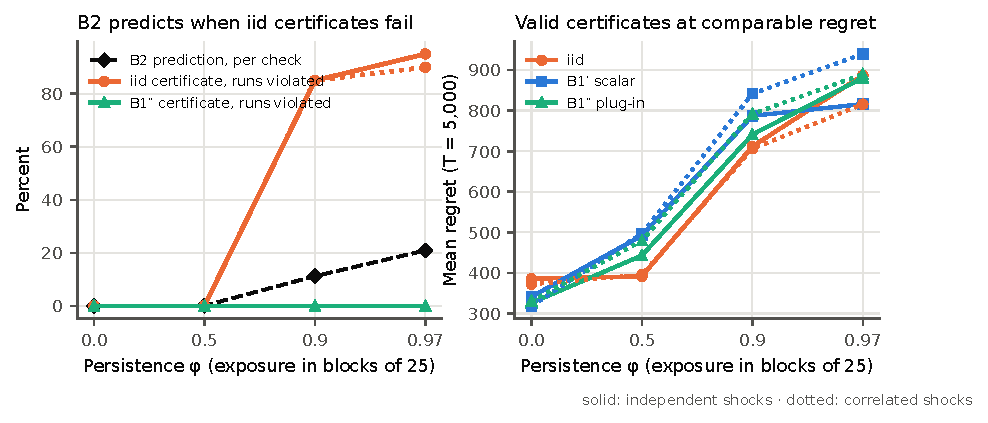
\includegraphics[width=\linewidth]{../figures/f3_b2_bridge.pdf}
\caption{Left: B2's predicted per-check miscoverage and the observed share of runs with a violated iid certificate, blocks of 25. Right: mean regret of SP-UCB with iid, B1$'$ and B1$''$ certificates.}\label{fig:b2}
\end{figure}

\begin{table}[t]\centering\small
\begin{tabular}{lccccc}
\toprule
Exposure & $\varphi$ & Independent shocks: iid / B1 / B1$'$ & Correlated shocks: iid / B1$'$ / B1$''$ \\
\midrule
One at a time & 0 & 353 / 753 / \textbf{295} & 357 / 317 / \textbf{313} \\
One at a time & 0.5 & 457 / 752 / \textbf{396} & 460 / 383 / 412 \\
One at a time & 0.9 & 533 / 759 / 564 & 642 / 646 / \textbf{606} \\
One at a time & 0.97 & 649 / 755 / 679 & 693 / 683 / 760 \\
Blocks of 25 & 0 & 380 / 766 / \textbf{338} & 372 / 319 / 330 \\
Blocks of 25 & 0.5 & 406 / 916 / 510 & 395 / 497 / 479 \\
Blocks of 25 & 0.9 & 629$^\dagger$ / 1,023 / 818 & 706$^\dagger$ / 841 / 792 \\
Blocks of 25 & 0.97 & 853$^\dagger$ / 1,034 / 828 & 816$^\dagger$ / 939 / 889 \\
\bottomrule
\end{tabular}
\caption{Mean regret ($T=5{,}000$). $^\dagger$ iid certificate invalid in 75--95\% of runs. B1$'$ has no guarantee under correlated shocks; B1$''$ does. The independent-shock columns use unshuffled worlds and are from a separate sweep.}\label{tab:b1regret}
\end{table}

\paragraph{Findings.}
\begin{itemize}
\item \emph{B2 predicts the failure} (Prediction~\ref{pred:q3}a; Table~\ref{tab:b2}, Figure~\ref{fig:b2}). Blocks of 25 inflate the sample-mean standard deviation by 1.7, 3.5 and 4.4 at $\varphi=0.5$, 0.9, 0.97; the iid certificate is then violated in 0\%, 85\% and 90--95\% of runs. One-at-a-time exposure interleaves arms (repeat pulls about 20 rounds apart, correlation $\varphi^{20}\approx0.54$ at 0.97), so the inflation is small and the conservative union-bound level still covers.
\item \emph{Innovation certificates are always valid} (Prediction~\ref{pred:q3}b): B1, B1$'$ and B1$''$ were never violated in any of several thousand runs.
\item \emph{Tight certificates cost little} (Prediction~\ref{pred:q3}c; Table~\ref{tab:b1regret}). B1$'$ and B1$''$ remove most of B1's cost and beat iid pooling when persistence is low or exposure is interleaved (16\% lower regret at $\varphi=0$). They are 9--30\% worse under bursty exposure at $\varphi=0.5$--0.9, which is exactly where the iid certificate is invalid; regret does not reward validity there because the iid violations mostly under-cover suboptimal components.
\item \emph{Irrevocable decisions inherit the failure} (Prediction~\ref{pred:q3}d). Successive elimination with iid certificates wrongly eliminated the best arm in 35--90\% of bursty high-persistence runs, against a nominal 5\%; with innovation certificates, never. The price is caution: at these gaps (0.1--0.4 against unit fluctuation variance) valid certificates eliminate almost nothing within 5,000--20,000 rounds.
\end{itemize}

\answer{Persistence must enter confidence sets. Under bursty exposure, which is the norm for slates and batched updates, iid certificates are violated most of the time, in the amount B2 predicts, and irrevocable decisions built on them fail. Innovation-regression certificates are always valid, and their scalar versions cost little regret.}

%=====================================================================
\section{Q4. How should a learner act on persistent fluctuations?}\label{sec:q4}
%=====================================================================

\subsection{What theory says}

\paragraph{Joint filter.} Stacking long-run means and AR lags gives one Gaussian state that every observation updates for every arm and lag \src{S}. We verify the implementation against dense conditioning on the full node-time covariance.

\begin{proposition}[Innovation lower bound \src{S,P}]\label{prop:floor}
With stationary covariance $K_0$ and innovation covariance $Q_G$, every causal policy has dynamic regret at least $T\{\mathcal G(\mu,K_0)-\mathcal G(\mu,K_0-Q_G)\}$, $\mathcal G(\mu,K)=\E\max_i(\mu_i+Z_i)$.
\end{proposition}

\paragraph{Which uncertainty to explore.} Current-state Thompson sampling draws the fresh innovation, which no future observation will reveal; exploring it is pure cost. Predictive sampling \src{P} draws only the part that next round's rewards would reveal, $B=CV^{-1}C^\top$ with $C=\Cov(f_t,f_{t+1})$, $V=\Var(f_{t+1})$. Exploration of any kind pays only if enough future observations remain to use what it learns.

\begin{prediction}\label{pred:q4}
(a) Modelling dynamics beats iid policies on persistent data. (b) Current-state Thompson sampling underperforms policies that explore persistent uncertainty. (c) Predictive exploration beats greedy use of the model only when each arm receives enough future observations. (d) A graph-shrunk shock covariance improves decisions only where Q1 found community-specific shocks.
\end{prediction}

\subsection{Evidence: a controlled benchmark}

\paragraph{Design.} 100 arms on a $10\times10$ grid; AR(20) coefficients proportional to $e^{-r/6}$ summing to 0.97; shocks correlated along the grid ($(I+5L)^{-1}$, unit diagonal); smooth long-run means; observation sd 0.3; $T=2{,}000$; 8 seeds; variants with weak persistence (0.6) and with independent shocks. Model-based policies know the dynamics; means are unknown.

\begin{figure}[t]\centering
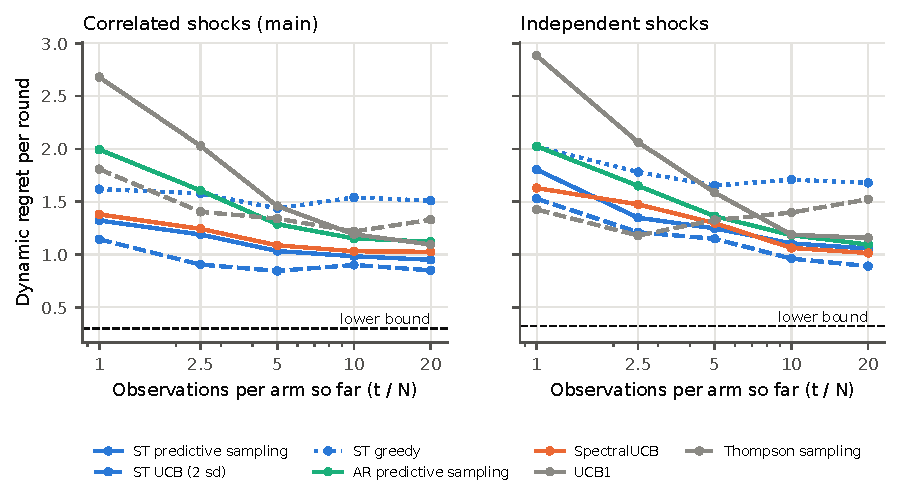
\includegraphics[width=\linewidth]{../figures/f4_toy_curves.pdf}
\caption{Benchmark: average dynamic regret over the first $t$ rounds (main configuration, left; independent shocks, right). Dashed: innovation lower bound.}\label{fig:toy}
\end{figure}

\begin{table}[t]\centering\small
\begin{tabular}{llccc}
\toprule
Policy & Models & Main & Independent shocks & Weak persistence \\
\midrule
ST UCB, 2 sd (tuned) & both channels & \textbf{0.850} & \textbf{0.890} & 1.856 \\
ST predictive sampling & both channels & 0.950 & 1.057 & 1.568 \\
SpectralUCB & mean channel only & 1.026 & 1.014 & 1.953 \\
UCB1 & nothing & 1.095 & 1.157 & 1.867 \\
AR predictive sampling & persistence only & 1.121 & 1.094 & \textbf{1.525} \\
ST current-state TS & both channels & 1.258 & 1.452 & 2.246 \\
Thompson sampling & nothing & 1.329 & 1.523 & 1.675 \\
ST greedy & both channels & 1.509 & 1.678 & 1.932 \\
\midrule
Innovation lower bound & & 0.298 & 0.323 & 1.276 \\
\bottomrule
\end{tabular}
\caption{Benchmark: dynamic regret per round at $T=2{,}000$.}\label{tab:toy}
\end{table}

\paragraph{Findings.} Joint predictive sampling, which has no tuning parameter, cuts dynamic regret 27\% against Thompson sampling and 13\% against UCB1, closing 37\% of the gap to the lower bound (tuned UCB closes 46\%; its multiplier was chosen on the same runs). Mis-targeted exploration is as harmful as having no model: greedy, current-state Thompson sampling and the theory-constant UCB all lose to UCB1 (Prediction~\ref{pred:q4}b). Predictive sampling leads greedy at every horizon in Figure~\ref{fig:toy}, because priors are weak and each arm receives 20 observations. Correlated shocks add 15\% on top of persistence (joint against persistence-only predictive sampling); with independent shocks the gain disappears (Prediction~\ref{pred:q4}d). Here fluctuations dominate the decision: their standard deviation (1.0) is twice the spread of long-run means (0.5). With weak persistence the lower bound is already high and all gains shrink.

\subsection{Evidence: two web platforms}

\paragraph{Designs.} \emph{KuaiRec daily:} 253 videos observed on all 63 days; reward the logit daily complete-play rate; ten slots per day; models fitted on the first $F\in\{28,35,42\}$ days; a sparse-history variant sees only ten videos per fit day. \emph{Wikipedia:} log daily views of 150 articles; ten featured slots per day; models fitted on a rolling 365-day window and tested on the next 120 days at three origins (January 2023, January 2024, December 2024); one-domain and six-domain panels. All panels assume that showing an item does not change its organic engagement.

\paragraph{KuaiRec daily.} Deviations persist (lag-1 autocorrelation 0.78) and are as large as the spread of long-run levels (sd 0.46 against 0.54). The panel is one upload cohort (median age 2 days at the start), whose engagement falls during days 21--42 (mean slope $-0.023$ per day) with heterogeneous level shifts of about 0.5, and then flattens. A stationary-mean model fitted through day 42 therefore reverts toward stale early-life levels, which is why the last observed value is the best rule at $F=42$ (0.93 regret per day against 1.31). A small likelihood-selected drift in the level gives the best average (2.36).

\begin{table}[t]\centering\small
\resizebox{\linewidth}{!}{%
\begin{tabular}{lcccc}
\toprule
Policy (regret per day) & KuaiRec full & KuaiRec sparse & Wikipedia one domain & Wikipedia six domains \\
\midrule
Model, greedy & 2.41 & 3.93 & 0.441 & 1.327 \\
Model + drift, greedy & \textbf{2.36} & -- & \textbf{0.376} & 1.257 \\
Model, UCB 1 sd & 2.57 & \textbf{3.59} & 0.436 & \textbf{1.205} \\
Model, predictive sampling & 4.04 & 6.85 & 0.407 & 1.470 \\
Temporal-only model, greedy & 2.44 & -- & 0.448 & 1.309 \\
Last observed value & 2.88 & -- & 0.486 & 1.434 \\
iid Thompson sampling & 3.90 & 6.35 & 0.553 & 1.588 \\
\midrule
Graph in shock covariance: real / rewired / none & 2.63 / 2.64 / 2.62$^*$ & -- & 0.441 / 0.441 / 0.441 & 1.327 / 1.307 / 1.299 \\
\bottomrule
\end{tabular}}
\caption{Web platforms, regret per day. KuaiRec: mean over $F\in\{28,35,42\}$ (5 seeds for stochastic policies). Wikipedia: mean over three origins and 5 noise seeds. Graph row: greedy policies, except $^*$persistent sampling on KuaiRec. On six domains, community blocks give 1.290 (greedy) and 1.456 (predictive sampling, against 1.500 with the common factor).}\label{tab:web}
\end{table}

\paragraph{Wikipedia.} On one domain, attention persists with a weekly cycle (lag-1 autocorrelation 0.72, lag-7 0.74) and the oracle's top ten is stable (1--6\% daily turnover, gap between the 10th and 11th article 0.07--0.21). Most regret comes from one window: in January 2024, 12.6\% of each day's top ten were articles outside the fit window's top ten, against 1.3\% a year earlier. The drifting-level filter cuts regret 32\% against iid Thompson sampling and predictive sampling 26\%. On six domains, rankings turn over far faster (22\% per day; gap 0.03) because game days rotate which teams lead. Every model beats iid Thompson sampling (best: $-24\%$), and mild optimism (UCB, 1 sd) is the best policy.

\paragraph{Does the graph help decisions where it carries shocks?} Only slightly. On six domains, where hyperlinks carry community shocks and fit held-out shocks best (Table~\ref{tab:shocks}), putting them into the shock covariance changes regret by $-2.0\%$ under predictive sampling ($\pm1.3\%$ s.e., 15 paired runs) and by $+2.2\%$ under greedy ($\pm1.1\%$); community blocks give $-2.9\%$ and $-0.7\%$ (Figure~\ref{fig:wikimulti}). Neighbours predict shocks about as well as in the benchmark ($R^2$ 0.36 against 0.46), so the difference lies elsewhere: on Wikipedia, which articles lead is set mostly by long-run levels (fluctuation sd 0.48 against level spread 0.91), whereas in the benchmark fluctuations dominate (sd 1.0 against 0.5). Sharper beliefs about today's shocks rarely change the top ten when levels decide it.

\begin{figure}[t]\centering
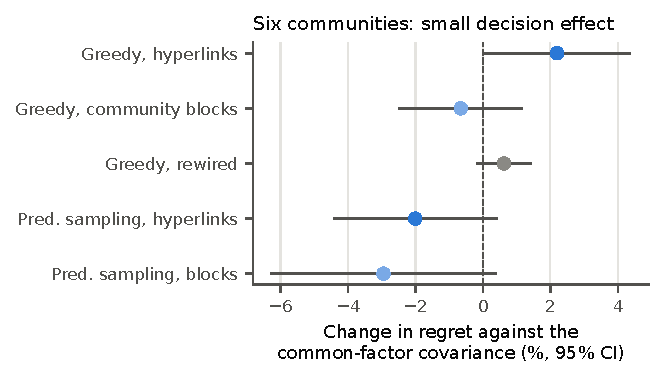
\includegraphics[width=0.55\linewidth]{../figures/f6_wikipedia_multi.pdf}
\caption{Six-domain Wikipedia: change in regret from a graph-shrunk shock covariance against a common-factor covariance, paired by origin and noise seed (95\% intervals).}\label{fig:wikimulti}
\end{figure}

\subsection{Synthesis: when does exploration pay, and when does the graph help?}

\begin{figure}[t]\centering
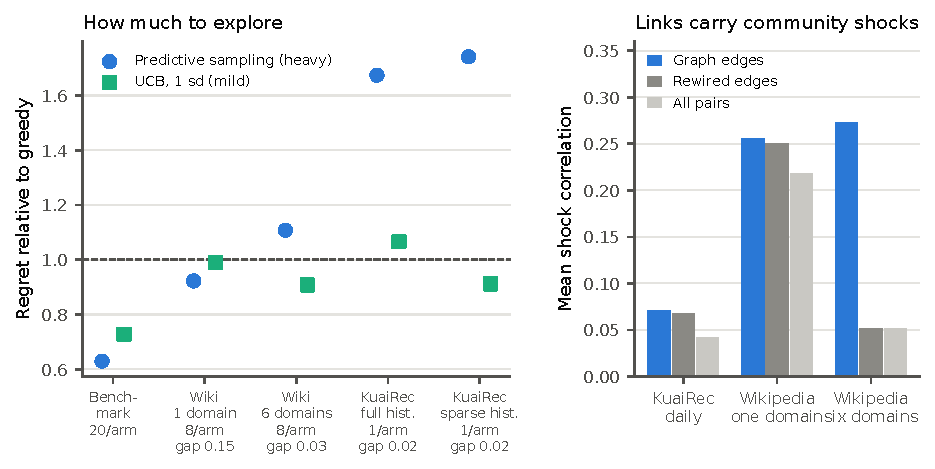
\includegraphics[width=\linewidth]{../figures/f5_synthesis.pdf}
\caption{Left: predictive sampling relative to greedy use of the same model, against the number of future observations each arm receives. Right: value of the graph in the shock covariance (held-out log-likelihood gain over a common-factor model) on the three daily panels.}\label{fig:synth}
\end{figure}

Table~\ref{tab:synth} lines up the five environments.

\begin{table}[t]\centering\small
\resizebox{\linewidth}{!}{%
\begin{tabular}{lccccccc}
\toprule
Environment & Future obs. per arm & 10th--11th gap & Daily top-10 turnover & Fluctuation / level sd & Pred. sampling / greedy & UCB 1 sd / greedy & Best model / iid TS \\
\midrule
Benchmark & 20 & -- & -- & 2.0 & \textbf{0.63} & 0.73 & 0.71 \\
Wikipedia, one domain & 8 & 0.15 & 3\% & 0.39 & \textbf{0.92} & 0.99 & 0.74 \\
Wikipedia, six domains & 8 & 0.03 & 22\% & 0.52 & 1.11 & \textbf{0.91} & 0.76 \\
KuaiRec daily, full history & 1.1 & 0.02 & 33\% & 0.85 & 1.67 & 1.07 & 0.62 \\
KuaiRec daily, sparse history & 1.1 & 0.02 & 33\% & 0.85 & 1.74 & \textbf{0.91} & 0.56 \\
\bottomrule
\end{tabular}}
\caption{When exploration pays. Ratios below 1 favour the exploring policy over greedy use of the same model.}\label{tab:synth}
\end{table}

\paragraph{What the synthesis shows.}
\begin{itemize}
\item \emph{Modelling dynamics always pays}: the best model-based policy has 24--44\% less regret than iid Thompson sampling in every environment (Prediction~\ref{pred:q4}a).
\item \emph{How much to explore depends on observations per arm and on gaps} (Prediction~\ref{pred:q4}c, refined). Heavy exploration of persistent uncertainty (predictive sampling) beats greedy only where arms receive many observations and the top is well separated or dominated by fluctuations (benchmark, one-domain Wikipedia). With near-ties and fast turnover it shuffles near-equal items at a cost, even with eight observations per arm (six-domain Wikipedia). Mild optimism helps wherever priors are weak or rankings move (benchmark, six-domain Wikipedia, sparse KuaiRec) and is roughly neutral otherwise; with strong priors and about one observation per arm (full-history KuaiRec), greedy is best.
\item \emph{The graph helps the fluctuation channel in proportion to how much fluctuations decide the ranking} (Prediction~\ref{pred:q4}d, refined): 15\% in the benchmark, where fluctuations dominate; at most $\pm3\%$ on six-domain Wikipedia, where links carry shocks but levels decide the top ten; nothing where shocks are not community-specific.
\end{itemize}

\answer{Model the dynamics: it is the largest and most consistent gain on real data (24--44\% less regret than iid Thompson sampling everywhere). Explore only uncertainty that persists, and match the amount to the setting: heavy exploration when arms receive many observations and the top is well separated, mild optimism when priors are weak or rankings turn over, greedy use of the model when priors are strong and observations per arm are few. A graph belongs in the shock covariance only when shocks are community-specific, and it pays only to the extent that fluctuations, rather than long-run levels, decide which items lead.}

%=====================================================================
\section{Lessons, limitations and open problems}
%=====================================================================

\paragraph{A checklist for practitioners.}
\begin{enumerate}
\item \emph{Measure before trusting.} Compare each candidate graph with its rewiring on held-out data: neighbour agreement after removing popularity (mean channel) and held-out likelihood of shocks (fluctuation channel).
\item \emph{Certify pooling.} Uncertified pooling wins on average and fails on informative graphs exactly where a best item sits in a weaker community. Use certificates, and expect gains in proportion to the components they can reject.
\item \emph{Account for persistence in every confidence statement,} especially when exposure is bursty. Use innovation-regression certificates for any irrevocable decision.
\item \emph{Model dynamics, target exploration.} Explore persistent uncertainty only; use heavy exploration when arms will be observed often and gaps are clear, mild optimism when rankings move, and the model greedily when priors are strong.
\item \emph{Check what decides the ranking.} If long-run levels dominate fluctuations, a graph in the shock model will barely change decisions even when it fits shocks better.
\end{enumerate}

\paragraph{Limitations.} KuaiRec ground truth uses one watch ratio per user--video pair, which understates preference alignment. Panel experiments assume that showing an item does not change its organic demand. Dynamics are estimated in a fit window and then treated as known. The benchmark fixes the model class, while real engagement shows cohort drift outside it. Regret bounds for B1$'$ and B1$''$ under correlated shocks are stated through realized information.

\paragraph{Open problems.} (1) A valid and narrow certificate for the mean channel on real graphs; level-matched calibration closes about half of the gap to the oracle. (2) Per-pull information constants under correlated shocks, and the path rate of graph-design elimination under persistence. (3) Learning dynamics online while keeping certificates valid. (4) Drift models for engagement lifecycles. (5) Testing community-specific shocks on platforms with live feedback.

\appendix

%=====================================================================
\section{Proofs of the bridging results}\label{app:proofs}
%=====================================================================

\paragraph{B1 (Theorem~\ref{thm:b1}).} Define $U_i=\hat\mu_i+\beta_t\|e_i\|_{J_t^{-1}}$ and $U_c=\min\{\max_{i\in C_c}U_i,\min_{w\in\Delta(C_c)}(w^\top\hat\mu+\beta_t\|w\|_{J_t^{-1}})+\varepsilon_c\}$. \emph{Validity:} Theorem~\ref{thm:innov} holds for all contrasts simultaneously, hence for every $e_i$ and every $w$ in every simplex; for $w\in\Delta(C_c)$, $w^\top\mu\ge v_c-\varepsilon_c$, so both terms of $U_c$ bound $v_c=\max_{i\in C_c}\mu_i$. Minimizing over $w$ is free because the event does not depend on $w$. \emph{Regret:} if $c$ is selected at round $t$, then $\mu^\star\le U_c\le v_c+\varepsilon_c+2\beta_t\|w\|_{J_t^{-1}}$, so $\min_w\|w\|^2_{J_t^{-1}}\ge(\Gamma_c-\varepsilon_c)^2/(4\beta_t^2)$; the information-growth condition makes this at most $1/(\iota_c(N_c-1))$. Arms are identical, and summation follows Theorem~\ref{thm:spucb}. \emph{AR(1) constant:} with independent arms the information is diagonal. The coefficient of $\mu_i$ in a pull of arm $i$ is $1-\varphi^hs$, where $h\ge1$ is the gap since the arm's last observation and $s\in[0,1]$ is the filter's estimate after unit residuals (each filter step is a convex combination of $\varphi$ times the previous estimate and the new residual), so it is at least $1-\varphi$; the predictive variance is at most $V+r$.

\paragraph{B1$'$ (Proposition~\ref{prop:b1p}).} With $Q_G$ diagonal and $H=\alpha I$, each $u_t$ has one nonzero entry, so each arm's score $W_i=\sum_{t:a_t=i}u_t\epsilon_t$ is a scalar martingale with quadratic variation $\I_{ii}$. The one-dimensional method of mixtures gives $|W_i|\le\sqrt{2J_{ii}\log(\sqrt{J_{ii}/\alpha}/\delta')}$ at all times with probability at least $1-\delta'$; the regularization bias is at most $\sqrt\alpha$. The pooled statistic $q_c/J_c$ with $J_c=\alpha+\sum_{i\in C_c}\I_{ii}$ estimates the information-weighted average of the pulled arms' means, which is at least $v_c-\varepsilon_c$, with a scalar martingale error. A union bound over $N+M$ statistics with $\delta'=\delta/(N+M)$ completes the proof.

\paragraph{B1$''$ (Proposition~\ref{prop:b1pp}).} Let $G=J-\alpha I$. Then $q_i-\sum_{j\ne i}G_{ij}m_j=G_{ii}\mu_i+\sum_{j\ne i}G_{ij}(\mu_j-m_j)+W_i$, where $W_i=\sum_tu_{t,i}\epsilon_t$ is a scalar martingale with quadratic variation $G_{ii}$. On the event $E$ that all scalar mixture bounds hold, and given intervals $[l_j,h_j]\ni\mu_j$ with midpoints $m_j$ and half-widths $\rho_j$, the error of $\hat\mu_i=(q_i-\sum_{j\ne i}G_{ij}m_j)/J_{ii}$ is at most $(\sqrt{2J_{ii}\log(\sqrt{J_{ii}/\alpha}/\delta')}+\alpha+\sum_{j\ne i}|G_{ij}|\rho_j)/J_{ii}$. Starting from $[0,1]$, which contains the truth, induction keeps every interval true-containing on $E$. For components, write $\mu_i=\theta_c+d_i$ with $\theta_c$ the midrange and $|d_i|\le\varepsilon_c/2$; the design $P^\top u_t$ ($P$ the membership matrix) gives the same argument for $\theta$, with a deterministic deviation term $\sum_i|(P^\top G)_{ci}|\varepsilon_{c(i)}/2$, so $\hat\theta_c+\rho_c+\varepsilon_c/2\ge v_c$. With independent shocks $G$ is diagonal, the cross terms vanish and the deviation term equals $\varepsilon_c/2$ times the information, recovering SP-UCB's structure. In implementation, upper bounds must not be clipped at 1, since ties created by clipping are broken by index.

\paragraph{B2 (Proposition~\ref{prop:b2}).} Within a block of $b$ consecutive pulls the autocovariances are $V\varphi^{|s-u|}$; summing gives $\Var(\sum)=V[b\frac{1+\varphi}{1-\varphi}-\frac{2\varphi(1-\varphi^b)}{(1-\varphi)^2}]$. Blocks separated by other arms' blocks are nearly independent, so $n$ pulls in blocks have variance $(V/n)f(b,\varphi)$. The sample mean is Gaussian, giving the stated miscoverage.

\paragraph{B3 (Proposition~\ref{prop:b3}).} Part (1): after the initial lags, the full-field innovation transform $X_t-\sum_k\mathrm{diag}(a_k)X_{t-k}=D_c\mu+\eta_t$ adds information $D_cQ_G^{-1}D_c$ per field \src{S}; substituting this information for the count-based information in the change-of-measure program of \src{A} replaces $\sigma^2$ by $q/c^2$. Part (2) is the Gaussian variance of a contrast of two arms observed in the same round.

%=====================================================================
\section{Data and graph construction}\label{app:data}
%=====================================================================

\paragraph{KuaiRec.} Small matrix: 1,411 users $\times$ 3,327 videos, 4,676,570 interactions, 17,827 blocked pairs. Big matrix: 7,176 $\times$ 10,728, 12,530,806 interactions; no overlap with the small matrix. Social network: 472 users, 146 in the evaluation set, 47 edges among them. Reward R1 $=\min(\text{watch ratio},5)/5$ (median watch ratio 0.77; 4.6\% above 2); R3 counts a watch ratio above 2 as a like. Graphs are union-$k$NN; Laplacians are scaled to mean degree one; nulls are degree-preserving rewirings and Erd\H{o}s--R\'enyi graphs. U-coeng: Jaccard on fully watched non-evaluation videos. U-coeng-idf and U-coauthor: cosine on IDF-weighted engagement by video or by creator. U-mf and I-mf: PureSVD (rank 64) on leakage-free splits. U-cotag: per-tag taste. U-cotime: hour-of-day profile. U-feat, U-geo (same city 1, province 0.3), U-demo: profile fields. I-coeng: IDF-weighted engagement from non-evaluation users. I-coauthor: same creator. I-tag, I-cat: tags and three-level categories.

\paragraph{Wikipedia.} Public Wikimedia REST API (daily user page views, all access, 2022--2025) and MediaWiki links API. One domain: the 150 most-viewed articles linked from ``List of programming languages'' with complete data (512 of 691), 3,037 hyperlinks. Six domains: 25 articles each from NFL teams, NBA teams, MLB teams, Premier League clubs, UN member states and programming languages, 1,990 hyperlinks (84\% within a domain).

%=====================================================================
\section{Reproducibility}\label{app:repro}
%=====================================================================

{\footnotesize
\begin{verbatim}
python -I experiments/kuairec/{data,graphs,alignment}.py        # Q1, mean channel
python -I experiments/kuairec/setting_a.py | setting_a2.py | setting_b.py   # Q2
python -I experiments/st_toy/coverage.py --tag {_v2,_elim,_scalar,_plugin}  # Q3
python -I experiments/st_toy/toy.py [--extra]                   # Q4 benchmark
python -I experiments/kuairec/daily.py [--extra | --sparse]     # Q4 KuaiRec
python -I experiments/wikipedia/collect.py; collect_multi.py    # Wikipedia data
python -I experiments/wikipedia/attention.py [--dataset multi] [--diagnose]
python -I experiments/deepdive.py                               # theory-to-data analyses
python -I experiments/paper_figures_v2.py                       # figures
\end{verbatim}}

\end{document}
